\documentclass[a4paper,12pt]{article}
\usepackage[a4paper,left=3cm,right=3cm,top=3cm,bottom=3cm]{geometry}
\usepackage{setspace}
%\renewcommand{\baselinestretch}{2}

\usepackage[utf8]{inputenc}

\usepackage[USenglish]{babel}
\usepackage[babel]{csquotes}

\usepackage{amsmath, amssymb}

\usepackage[colorlinks=true, allcolors=blue]{hyperref}
\usepackage[all]{hypcap}

\usepackage{graphicx, subcaption}
\usepackage{tabularx}

\usepackage[style=authoryear, date=year, maxbibnames=100, backend=biber, natbib]{biblatex}
\bibliography{~/Zotero/Bibliothek.bib}
%% APPROXIMATING ASA STYLE (Amercan Sociological Association)
% remove comma after last author and add colon before cited pages within text
\DeclareDelimFormat{nameyeardelim}{\space}
\renewcommand*{\postnotedelim}{\addcolon \addspace}
\DeclareFieldFormat{postnote}{\mknormrange{#1}}
% remove parentheses around year and add dots in bibliography
\usepackage{xpatch}
\xpatchbibmacro{date+extradate}{%
  \printtext[parens]%
}{%
  \setunit{\addperiod\space}%
  \printtext%
}{}{}
% implement volume and number in reference list as: volume(number)
\renewbibmacro{in:}{}
\renewbibmacro*{volume+number+eid}{%
  \printfield{volume}%
  \printfield{number}%
  \setunit{\addcomma\space}%
  \printfield{eid}}
\DeclareFieldFormat[article]{number}{\mkbibparens{#1}}
% place pages after colon without pp. in bibliography
\renewcommand*{\bibpagespunct}{\addcolon\space}
\DeclareFieldFormat{pages}{#1}


\title{A socio-economic Model of Segregation, Residential Mobility and Housing Inequality\footnote{
I want to thank Johanna Mehltretter, Hannah Reitz, Max Otto, Marcel Kappes and my supervisors Thomas Gautschi and Michael Mäs for comments and feedback during multiple stages of this project.

This project has been presented at the CDSS Workshop at the University of Mannheim, the 14th Annual INAS Conference 2022 in Florence, the 16th Annual INAS Conference 2024 in Leipzig, the Analytical Sociology Workshop 2024 in Venice, and the ASA Annual Meeting 2025 in Chicago. I want to thank all attendees and commentators of these events for their attention and comments.

This work was supported by the University of Mannheim’s Graduate School of Economic and Social Sciences. The simulations of the computational model have been performed on the HELIX high performance computing cluster funded by the German federal state of Baden-Württemberg.

In memory of Jürgen Friedrichs.}}

\author{Malte Grönemann \\ University of Mannheim, Germany \\ \texttt{malte.groenemann@uni-mannheim.de}}

\begin{document}

\maketitle

\textcolor{red}{WORKING PAPER: Do not distribute or cite without permission}

You find the supplementary material on the \href{https://osf.io/nqazw/?view_only=5d2358955d9542de921be4966ffe006c}{OSF project page}.

\begin{abstract} 
Landlords have been largely overlooked in research on segregation, neighborhoods and housing inequality. However, they have significant agency about the type and quality of housing in a given area. Given that households often value properties of housing units more than properties of the neighborhood and that housing is unequally distributed in space, existing theories likely misrepresent how and why residential segregation emerges and neighborhoods form. In this article, I present a theoretical model of the housing market that considers both the preferences and decisions of households as well as the agency of landlords. Based on three empirically grounded assumptions (households value the quality of a housing unit and the status of the neighborhood while landlords invest in their units when rents in the neighborhood rise), I can unify and explain multiple phenomena in urban sociology, such as the emergence and stability of segregated neighborhoods and patterns of inequalities in residential mobility, housing and neighborhood quality, as well as housing affordability.
\end{abstract}


\newpage

\section{Introduction}

It appears evident that more affluent households live in larger, better houses and more desirable neighborhoods. However, while some characteristics of a neighborhood are based on geography (e.g., waterfronts, elevation) and infrastructure (e.g., commuting time to the workplace), most features that make a neighborhood more or less attractive are a result of the people living in that neighborhood: which shops and restaurants supply the local population? How good is the quality of the local school? What is the crime rate in the neighborhood? Sociologists have therefore described neighborhood formation as an archetype of a \textit{self-organizing process} \citep{schellingDynamicModelsSegregation1971, galsterNatureNeighbourhood2001, fossettEthnicPreferencesSocial2006}. Neighborhoods form from the people that inhabit an area but also shape their daily surroundings and whom they interact with to an extent that shapes their opportunities for life \citep{sampsonAssessingNeighborhoodEffects2002, sharkeyWhereWhenWhy2014, chettyImpactsNeighborhoodsIntergenerational2018a} and subsequent generations \citep{sharkeyIntergenerationalTransmissionContext2008}. As neighborhoods change, they become more or less attractive to both potential new residents and existing residents. The resulting residential mobility can reproduce features of the neighborhood or massively change its local culture and social structure when change reaches a tipping point.

Existing theoretical models of residential segregation and neighborhood formation have explained these phenomena based on local amenities and the preferences of people who they (or do not) want to be their neighbors. Such preferences, combined with income and wealth inequality, lead households with different socio-economic characteristics to sort themselves into distinct neighborhoods, while poorer households are priced out of the most desirable neighborhoods. These models often (implicitly) assume that the type and quality of housing follow such developments. Nevertheless, there is reason to doubt that these models tell the whole picture. Empirical research indicates that households are primarily concerned with finding a place that meets their needs and is affordable. Characteristics of housing units are more important to them than characteristics of the neighborhood \citep{chauCriticalReviewLiterature2003, bayerEquilibriumModelSorting2004, mummoloWhyPartisansNot2017, delucaNotJustLateral2020}. Moreover, changes in the housing stock are a defining feature of neighborhood change \citep{redfernWhatMakesGentrification2003}. Are the characteristics of the housing units and the agency of those who can change these characteristics (i.e., owners and landlords) not important in explaining residential segregation, neighborhood change, or patterns of inequality? I am not the first to observe this omission. For example, \citet[1081]{rosenthalChangePersistenceEconomic2015} note that "there are important dynamic links between maintenance and neighborhood change although that relationship has mostly escaped attention in the literature" and \citet[1093]{desmondPoorPayMore2019} constitute that landlords are "[c]onspicuously absent from most accounts of neighborhood dynamics or inequality."

Any description of a market is guaranteed to be incomplete if it only discusses one type of market actor, in this case, demand. While the supply side of the housing market, like landlords and real estate agents, has recently gained attention in sociological research in its own right (e.g., \cite{korver-glennCompoundingInequalitiesHow2018, desmondPoorPayMore2019, rosenRacialDiscriminationHousing2021}), this paper aims to combine supply and demand in a theoretical model to explain key workings and patterns in the fields of residential segregation, neighborhoods, residential mobility and housing inequality. The model additionally aims to synthesize and unite these related but previously often unconnected fields \citep{hwangThingsChangeThings2016}. My theoretical model makes three substantial assumptions: households prefer high-quality housing units and prefer to live next to high-status neighbors. Landlords invest in improving the quality of their housing if average rents in the neighborhood increase. If landlords do not invest, the quality of housing decays over time. The model explains the emergence of distinct neighborhoods through a self-reinforcing dynamic: when a neighborhood increases in status, it also becomes more desirable, leading to higher rents and increased investment by landlords. Because the attractiveness of the neighborhood rises with status and housing quality, rents increase further after the investment in housing quality, and poor, typically low-status residents are replaced with more affluent households. This cycle continues until a spatial equilibrium is reached, which aligns well with the reviewed descriptions of gentrification. In equilibrium, the model reproduces several stylized facts from urban research, generating stable and segregated neighborhoods by income, social status, and housing quality. Low-income residents exhibit significantly higher residential mobility, as they are frequently forced to relocate due to affordability issues. They live in lower-quality housing units and neighborhoods, and pay a larger share of their income for housing. As households with low social status reduce the attractiveness of a neighborhood by themselves, they typically live in worse housing conditions than higher-status households with the same income, because landlords invest based on local developments in rents.

The following section summarizes the empirical literature on residential segregation, neighborhoods, and housing inequality to identify the stylized facts that the model should be able to explain. The third section discusses existing theories and their shortcomings, which motivate the development of this new theory. Section four describes the micro-level assumptions of my theoretical model, motivating them with empirical literature on household preferences and real estate investment. Section five describes the dynamics and equilibrium results that these assumptions create in realistic conditions. Before concluding in section seven, I discuss the omissions and limitations of my model in section six.


\section{Review of the Empirical Literature}

This article aims to unify the literature on residential segregation and neighborhood change in a theoretical model. As such, the model shall be able to explain key stylized facts. A stylized fact is an empirical regularity that abstracts from and lightly theorizes many empirical observations into a general empirical claim especially worthy of explanation \citep{hirschmanStylizedFactsSocial2016}. In this section, I review significant lines of inquiry in urban sociology, demography, and economics to obtain stylized facts about social and economic segregation and its dynamics. However, as most reviewed research considers North America and Europe, the stylized facts and subsequent model will characterize patterns in market democracies. The applicability to other contexts may be possible but would require caution. The stylized facts and the theoretical model will not apply to contexts where housing is not allocated via markets. 


\subsection{Residential Segregation}

Residential segregation refers to the unequal distribution of population characteristics over residential areas beyond random chance \citep{masseyDimensionsResidentialSegregation1988, reardonNewApproachMeasuring2006}. Inequality or heterogeneity within a concept is a necessary condition for segregation. This unequal distribution of population groups in space can have different levels \citep{oecdDividedCitiesUnderstanding2018}, forms \citep{masseyDimensionsResidentialSegregation1988} and geographic scales \citep{leeCensusTractPatterns2008}. Although measurement of segregation is often difficult and relies on arbitrary spatial units \citep{reardonNewApproachMeasuring2006, leeCensusTractPatterns2008, leung-gagneItSurprisinglyDifficult2023}, neighborhoods are usually more homogenous concerning their population compared to entire cities.

Almost every feature of populations is distributed unequally within cities, and this observation holds globally, even though there are considerable differences in levels of segregation between countries and cities \citep{quillianSocioeconomicSegregationLarge2016, oecdDividedCitiesUnderstanding2018, vanhamUrbanSocioEconomicSegregation2021}. Sociologists have given most attention to segregation by race/ethnicity \citep{charlesDynamicsRacialResidential2003}. However, urban populations are also more or less segregated by income and wealth (e.g., \cite{reardonIncomeInequalityIncome2011, oecdDividedCitiesUnderstanding2018, helbigHinterFassadenZur2023}), age and household composition (e.g., \cite{owensInequalityChildrenContexts2016, loganBirdsFeatherSocial2016, mutganIncomeInequalityResidential2023}), education and socio-economic status (e.g., \cite{quillianSocioeconomicSegregationLarge2016, helbigHinterFassadenZur2023}), and political opinion and party preference (e.g., \cite{mummoloWhyPartisansNot2017}). 
Relatedly, the type of building and tenure (e.g., \cite{loufPatternsResidentialSegregation2016, oecdDividedCitiesUnderstanding2018, owensBuildingInequalityHousing2019}) and housing quality concerning size and amenities of the housing units themselves (for a review, see \cite{chauCriticalReviewLiterature2003}) and of the neighborhood like parks, waterfronts, distance to the center and public transport or disamenities like noise or air pollution are unequally distributed in space (e.g. \cite{leeNaturalAmenitiesNeighbourhood2018, heblichEastSideStoryHistorical2021, ruttenauerEnvironmentalInequalityResidential2021}).

Levels of income segregation have risen over the last decades (e.g., \cite{jargowskyTakeMoneyRun1996, reardonIncomeInequalityIncome2011, vanhamUrbanSocioEconomicSegregation2021}. The standard model of the spatial distribution of income has been that of a monocentric city with poor city centers and affluent suburbs \citep{bruecknerLecturesUrbanEconomics2011, rosenthalChangePersistenceEconomic2015}. While this is a good description of most US cities, this model does not hold globally \citep{bruecknerWhyCentralParis1999, quillianSocioeconomicSegregationLarge2016, gaigneWhoLivesWhere2022}. Inequality is a necessary condition for segregation, of course. However, more unequal countries and cities also tend to be more segregated cross-sectionally \citep{quillianSocioeconomicSegregationLarge2016, oecdDividedCitiesUnderstanding2018, vanhamUrbanSocioEconomicSegregation2021} and income segregation has risen as a result of increased income inequality \citep{reardonIncomeInequalityIncome2011, vanhamUrbanSocioEconomicSegregation2021, mutganIncomeInequalityResidential2023}. Segregation is predominantly a phenomenon of the extremes of the income distribution. The richest and, to a lesser extent, the poorest quantiles of the income distributions are most isolated in space (\cite{reardonIncomeInequalityIncome2011, quillianSocioeconomicSegregationLarge2016, oecdDividedCitiesUnderstanding2018, mutganIncomeInequalityResidential2023}). Families appear more economically segregated than households without children \citep{owensInequalityChildrenContexts2016, mutganIncomeInequalityResidential2023}.


\subsection{Neighborhood Stability and Change}

Most neighborhoods, especially at the very top and very bottom, maintain their position in the hierarchy of the city over long periods \citep{solariAffluentNeighborhoodPersistence2012, owensNeighborhoodsRiseTypology2012, rosenthalChangePersistenceEconomic2015}. Nevertheless, neighborhoods can change over time, although it is usually a highly localized and rare phenomenon \citep{solariAffluentNeighborhoodPersistence2012, owensNeighborhoodsRiseTypology2012, brown-saracinoExplicatingDividedApproaches2017}. Only a few neighborhoods within a city change at a time, if any at all. 

Gentrification has become the general term for the socio-economic ascent of a neighborhood \citep{owensNeighborhoodsRiseTypology2012}. Initially, gentrification was defined as the ascent of a previously lower-class neighborhood (typically near the city center) with below-average housing quality to a new middle- or upper-middle-class neighborhood with improved housing and infrastructure conditions accompanied by a new dominant lifestyle by an exchange of residents \citep{zukinGentrificationCultureCapital1987}. However, this term has been widened to include more and more diverse cases of neighborhood ascent \citep[530ff]{owensNeighborhoodsRiseTypology2012, brown-saracinoExplicatingDividedApproaches2017}. However, the narrow and wide definitions share that not only do the average incomes and rents in the neighborhood change but that they are associated with socio-cultural changes and changes in the built environment \citep{redfernWhatMakesGentrification2003}. More educated and affluent households with different lifestyles replace the initial residents. The businesses in the area increasingly cater to these new residents. Housing quality and public good provision increase \citep{zukinGentrificationCultureCapital1987}. Gentrification typically occurs in places of disinvestment within areas of at least some prosperity \citep{leyAlternativeExplanationsInnerCity1986, atkinsonEvidenceImpactGentrification2004} or in proximity to already established neighborhoods \citep{guerrieriEndogenousGentrificationHousing2013}.

\begin{figure}
\caption{The Gentrifying Neighbourhood over Time}
\begin{subfigure}{.5\textwidth}
  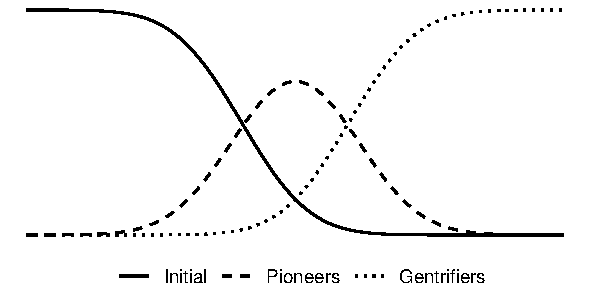
\includegraphics[width=\linewidth]{images/lit_01_stage_groups.pdf}
  \caption{Group Composition}
\end{subfigure}
\hfill
\begin{subfigure}{.5\textwidth}
  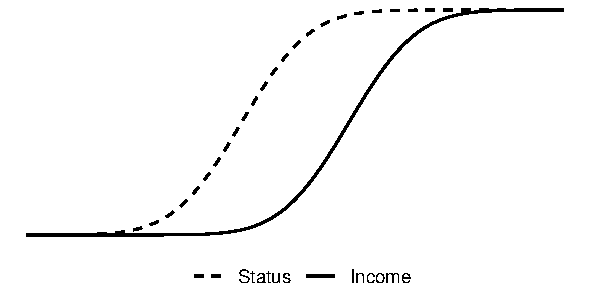
\includegraphics[width=\linewidth]{images/lit_01_stage_capital.pdf}
    \caption{Average Income and Status}
\end{subfigure}

\tiny{Schematic representation of a gentrifying neighborhood over time. (a) is adapted and simplified from \citet[70]{dangschatGentrificationHamburg1991}.}

\label{fig:gentri}
\end{figure}

Gentrification changes a neighborhood economically, socially and in terms of the built environment usually gradually but often fast compared to the usual stability of neighborhoods. The resulting sigmoid curve between two phases of relative stability is typical for neighborhood change \citep[927f]{meenSocialBehaviourBasis2003}. These changes in residents has been described in distinct successions of population groups. Before the beginning of the process of gentrification in a neighbourhood, residents are have low income and low status \citep{zukinGentrificationCultureCapital1987, dangschatGentrificationHamburg1991, blasiusPioneersGentrifiersProcess2016}. In the first stage of gentrification, \textit{pioneers} move in which have low income as well but have a higher socio-economic status. They are often students or creatives \citep{zukinGentrificationCultureCapital1987, blasiusPioneersGentrifiersProcess2016}. They in turn make the neighborhood more attractive, as they change the character and reputation of the neighborhood. The neighborhood then attracts \textit{gentrifiers} with more financial resources which drives up rents and investment. Figure \ref{fig:gentri} provides a schematic overview over this process. Crucially, the social changes of the neighborhood preceed the economic changes.

The literature often relates these successions of residents to forced displacement. However, differentiating between voluntary and forced moves is often complicated, and the amount of residential mobility associated with gentrification is typically low and varies by context \citep{freemanDisplacementSuccessionResidential2005, dingGentrificationResidentialMobility2016, leeGeographyGentrificationResidential2023}. Low-income households show high levels of residential mobility, independent of whether they live in gentrifying neighborhoods. Forced displacement might, therefore, not be necessary for gentrification dynamics; the characteristics of new residents change, but the vacancies are created by normal turnover \citep{freemanDisplacementSuccessionResidential2005}. The potential relationship of gentrification to displacement has spurred a large body of literature on the consequences of gentrification, especially for the displaced but also for the neighborhood and the city as a whole (for a review, see \cite{atkinsonEvidenceImpactGentrification2004}). 

In many ways, neighborhood descent constitutes the mirror image of gentrification, except that decline is a much slower process than ascent, primarily because housing decays at a slow rate \citep{glaeserUrbanDeclineDurable2005}. When a neighborhood declines, it is still attractive to some renters as they find cheap housing with amenities they could not afford elsewhere. As decline progresses, this holds only for continuously poorer households. There is again a replacement cycle where poorer households replace previous residents as infrastructure and housing quality decline. The population structure changes, but the population size does not necessarily decline \citep{guerrieriWithinCityVariationUrban2012}.


\subsection{Housing and Neighborhood Inequality}

Residential segregation and the spatial inequality of housing quality create distinct neighborhoods that affect their resident's lives. Unsurprisingly, the different dimensions of spatial inequalities are related: wealthier households inhabit housing units and neighborhoods of higher quality, whereas disadvantaged households have lower housing and neighborhood quality. Neighborhood inequalities, particularly concerning exposure to pollution and crime, children's school quality, and access to resources and opportunities, cause the reproduction of social inequalities over generations (e.g., \cite{masseyAmericanApartheidSegregation1993, sharkeyIntergenerationalTransmissionContext2008, chettyImpactsNeighborhoodsIntergenerational2018a}).

In recent years, increasing housing costs and stagnating incomes resulted in increasing financial burdens related to housing for low to middle-income households \citep{delucaHousingInsecurityPoor2022}. While more affluent households spend more on housing in absolute terms, poorer households spend a higher proportion of their income on housing. Absolute rent differences between poor and non-poor neighborhoods are small though \citep{desmondPoorPayMore2019}. For many low-income households, housing costs exceed the recommended maximum of 30\% of monthly income. A substantial share of the population even spends more than half their income on housing. In the US, African-Americans and Hispanics are more likely to be housing cost burdened \citep{delucaHousingInsecurityPoor2022}. 

Although they pay a large share of their income on housing, poor households frequently live in housing units with substantial quality issues, such as lacking heating or water, poor building materials, infestations, and mold. Poor households are also more likely to live in overcrowded units. In the US, living in substandard housing is especially prevalent for low-income families and racial minorities. Differences in housing quality between racial groups remain after controlling for income and minority households need more financial resources to attain the same residential outcomes \citep{crowderInterneighborhoodMigrationRace2010, delucaHousingInsecurityPoor2022}. 

Housing cost burdens and low housing quality are the prime reasons poor households have low housing security and high levels of residential mobility. Landlords (threaten to) evict tenants if they fall behind in rent payments, and tenants are forced to move when units fail to provide necessities. Poor households move often and on short notice. In contrast, affluent households move rarely, and if they do, they move to increase their residential satisfaction or because of life course events such as education, cohabitation, and childbirth \citep{bruchChoiceSetFormation2019, delucaNotJustLateral2020, delucaHousingInsecurityPoor2022}. These forced moves by low-income households often lead them to live in even worse units and neighborhoods, especially when households have been evicted \citep{desmondEvictedPovertyProfit2017, delucaHousingInsecurityPoor2022}. 


\subsection{Summary: Stylized Facts}

\begin{itemize}
\item Residents of a city are not evenly distributed in space. There is always segregation along social, economic, and demographic lines beyond what we expect by random chance.
\item The extremes of the income distribution are the most segregated groups.
\item Housing type and quality and other amenities are also unevenly placed.
\item These different spatial inequalities correlate with each other. Poorer residents typically have lower housing and neighborhood quality.
\item Disadvantaged residents have low housing security and high rates of residential mobility.
\item There is a negative relationship between income and the proportion of income spent on housing.
\item Neighborhoods maintain their rank within the city over long periods. Only a few neighborhoods change their relative position at a time, if at all.
\item Gentrification typically occurs close to established neighborhoods, amenities, or the city center.
\item Economic, socio-cultural, and infrastructural change in the city and neighborhoods are almost always linked. Social change precedes economic change in neighborhood ascent.
\item Gentrification can quickly change a neighborhood, whereas decline is usually slower as built infrastructure creates inertia.
\end{itemize}


\section{Explaining Urban Social Structure}


The reviewed stylized facts about residential segregation, neighborhood change, and housing inequalities (in North America and Europe) provide many interesting explananda for urban research. Indeed, many theories have been proposed to understand these patterns and dynamics. In this section, I will briefly review existing theories. As many theories share features, I have grouped them into families of theories and discuss their merits and shortcomings with specific reference to a few theories of the respective families. Lastly, I summarize my critique of these theoretical models and present my reasons for developing a new one.

Explanations for neighborhood change usually describe triggers that distort a spatial equilibrium, whereafter the described patterns of neighborhood change follow until the city settles into a new spatial equilibrium \citep{galsterNatureNeighbourhood2001}. For example, gentrification is connected to the overall economic situation, state-funded infrastructure investment, changing tastes and preferences, population growth, and changes in income distributions \citep{leyAlternativeExplanationsInnerCity1986, zukinGentrificationCultureCapital1987}. I am not going to review potential triggers that can set off neighborhood change or reasons spatial equilibria become unstable. I am concerned with theories that describe the reasons and the processes that lead to residential segregation. Such theories should be able to produce the reviewed stylized facts about neighborhood change when confronted with an exogenous shock to the spatial equilibrium. Unfortunately, such connections have been rare: "One way in which scholarship on gentrification has been limited is that it has generally remained isolated from the study of persistent poverty and segregation" \citep[227]{hwangThingsChangeThings2016}.


\subsection{Neighborhood Preferences}

There is a vast literature on theoretical models of residential segregation that explain segregation with households' preferences concerning their neighbors originating in urban ecology theory (for a review, see \cite{fossettEthnicPreferencesSocial2006}). Most of these models explain racial/ethnic segregation based on a preference for co-ethnic neighbors. As shown by \citet{schellingDynamicModelsSegregation1971}, such preferences lead to self-organization of segregation because individual moves create separate neighborhoods that realize the preferences of one group but not the other group. Moving into a neighborhood dominated by the outgroup does not improve residential satisfaction, even if the households prefer a more mixed neighborhood. Mixed neighborhoods are unstable, and high levels of segregation arise even with low levels of in-group favoritism.

However, some related models explain income segregation and more general patterns of social segregation as well. Such models assume that households prefer to live next to high-income neighbors (e.g. \cite{tieboutPureTheoryLocal1956, guerrieriEndogenousGentrificationHousing2013}) or that they value traits of their neighbors that are correlated with income (e.g. \cite{bayerEquilibriumModelSorting2004, fossettEthnicPreferencesSocial2006, benardWealthStatusBasedModel2007, yavasDissectingIncomeSegregation2019}). In these cases, different neighborhoods do not realize preferences for specific groups, but preferences are similar for all households, so the same neighborhoods are desirable for everyone. Segregation then arises because less affluent households can be outpriced. Households sort into the best neighborhoods they can afford. Such models can explain not only segregation by income but also the traits households have preferences over and those that correlate with income. Additionally, such models imply dynamics that closely mimic patterns of neighborhood change: when a neighborhood is becoming more attractive, poor residents are displaced by price increases and replaced by affluent in-movers. As more affluent neighbors have preferential characteristics, the neighborhood increases in attractiveness again. A self-reinforcing dynamic is created that continues until an increase in attractiveness no longer increases prices and the system reaches spatial equilibrium.

The main limitations of these models are that they fall short of the role of housing. Many models only consider preferences about neighbors (e.g., \cite{guerrieriEndogenousGentrificationHousing2013, yavasDissectingIncomeSegregation2019}). If the type and quality of the housing unit are unevenly distributed in space \citep{loufPatternsResidentialSegregation2016, oecdDividedCitiesUnderstanding2018, owensBuildingInequalityHousing2019} and preferences on housing characteristics are prioritized over preferences on the neighborhood \citep{chauCriticalReviewLiterature2003, bayerEquilibriumModelSorting2004, mummoloWhyPartisansNot2017, delucaNotJustLateral2020}, such models misrepresent the individual behavior leading to segregation. In the worst case, neighborhood preferences are not needed to generate segregation because of the uneven placement of more or less desirable housing units. Such models cannot explain the relationship between resident characteristics and housing quality. The models that consider preferences over housing units typically assume them to be exogenously given and fixed over time (e.g., \cite{bayerEquilibriumModelSorting2004, fossettEthnicPreferencesSocial2006, benardWealthStatusBasedModel2007}). While they can explain housing inequalities and better represent individual preferences, these models cannot explain the dynamics of housing quality. Changes in housing are a defining feature of neighborhood change \citep{zukinGentrificationCultureCapital1987, redfernWhatMakesGentrification2003} and therefore required in theories representing neighborhood change. Furthermore, the explanation of residential segregation by these models largely rests on the assumptions made about and does not explain the spatial distribution of housing quality.


\subsection{Amenities}

A typical family of explanations of both the spatial distribution of housing/neighborhood quality and socio-economic segregation is that more affluent households can outcompete poorer households for locations with the most amenities. Theories of this style have been influential in urban economics, particularly considering the relation of household income, housing unit size, and distance to the city center (see \cite{bruecknerLecturesUrbanEconomics2011}). In such models, housing is assumed to be cheaper with increasing distance to the central business district. Households can afford larger properties in suburbia at the expense of longer commutes. The choice of suburban living is made primarily by more wealthy families, causing an increase in household income and housing quality within a distance of the city center, while the poor live in small apartments in the city center. However, this concentric city model only performs well within the US \citep{bruecknerWhyCentralParis1999, quillianSocioeconomicSegregationLarge2016, gaigneWhoLivesWhere2022}. To quote \citet[55]{bruecknerLecturesUrbanEconomics2011}, "the urban model is less successful at explaining the locations of different income groups within the city than at predicting regularities in spatial structure such as the decline in building heights moving away from the CBD." This model also does not represent neighborhood change well.

\citet{bruecknerWhyCentralParis1999} propose a theory based on more amenities than commuting time to the central business district. They consider how the (exogenously given) spatial distribution of amenities like rivers, hills, waterfronts, parks, and historical buildings affect whether affluent households reside in the city center or the suburbs. They explain the pattern that many US cities have poor city centers and affluent suburbs. In contrast, European cities tend to have rich centers and poor outskirts because of the historically grown concentration of amenities in the old European city centers that counteract the suburbanization forces described above. However, the theory can account for many income segregation patterns depending on the spatial distribution of amenities. \citet{leeNaturalAmenitiesNeighbourhood2018, gaigneWhoLivesWhere2022} are examples of more recent theories based on exogenous amenities. 

Amenity-based theories assume, often implicitly, that housing units of higher quality are built in places that are attractive to affluent households. However, only the classic concentric model directly addresses why different housing is built in different spaces: land prices decline with distance to the city center. So, these models can explain the joint patterns of people and infrastructure and show how they reinforce each other to create stable arrangements in space, even if the supply side is rarely given much agency. Nevertheless, exogenous (dis)amenities are neither necessary nor sufficient for residential segregation. For example, \citet{heblichEastSideStoryHistorical2021} show that historical pollution patterns in England created socio-economic segregation with the poor living in the most polluted areas. They also show that the geographical pattern remained stable even decades after the pollution stopped (see also \cite{ruttenauerEnvironmentalInequalityResidential2021}). There is an asymmetrical effect of amenities. While the placement of amenities can explain where specific groups segregate, it cannot explain why socio-economic segregation persists after amenities change. Some amenity-based theories sometimes include endogenous changes in amenities due to population changes, like restaurants and shops that cater to these demographics (e.g., \cite{bruecknerWhyCentralParis1999}) that would explain the inertia in segregation patterns after changes in amenities. However, they still need to pay more attention to changes in housing stock and supplier's agency.


\subsection{Reasons for a new Theory}

In summary, many theories of segregation and neighborhood change focus on demand without (explicitly) considering supply. As housing preferences are more important than neighborhood preferences \citep{chauCriticalReviewLiterature2003, bayerEquilibriumModelSorting2004, mummoloWhyPartisansNot2017, delucaNotJustLateral2020} and housing is unequally distributed in space \citep{loufPatternsResidentialSegregation2016, oecdDividedCitiesUnderstanding2018, owensBuildingInequalityHousing2019}, such theories misrepresent segregation dynamics and neighborhood formation. 

Another key objective of my proposed theoretical model is to bridge the gap between residential segregation models and neighborhood change, as well as residential mobility and housing inequality. Despite their inherent connection, they are all phenomena generated by the housing market, and these research areas have remained mainly separate \citep{hwangThingsChangeThings2016}. Segregation represents stable patterns of neighborhood inequality, while neighborhood change involves rare transformations of single neighborhoods. The individual mobility behavior of residents creates segregation. The unequal placement of housing and households with different socio-economic characteristics in space implies that households with different characteristics live in housing units and neighborhoods of different quality.

By integrating these strands of literature, I aim to synthesize explanations of fundamental questions of urban research: Why do residents segregate into distinct neighborhoods? Why are neighborhoods so stable over time? Under what conditions do neighborhoods change? Why does neighborhood change follow typical patterns of invasion and succession of different socio-economic groups? Which residents move more frequently, and why? Who lives in housing units and neighborhoods of high and low quality? How much are households paying for housing?

Compared to existing theories, the model shall provide a more general explanation of multiple related phenomena. It shall be more realistic in its micro-foundations compared to models based on neighborhood preferences alone, acknowledging the agency of landlords and the importance of built infrastructure in households' decision-making about where to move.


\section{Micro-level Assumptions}

In the following, I propose a new theoretical model that includes supply to explain the joint patterns of the spatial distribution of population and built environment and their dynamics. I have formalized this theory in an agent-based model \citep{macyFactorsActorsComputational2002, axtellAgentBasedModelingEconomics2025}, based on the model by \citet{benardWealthStatusBasedModel2007}, which is a continuous variant of the famous model by \citet{schellingDynamicModelsSegregation1971}.  I will not consider exogenous amenities like waterfronts, elevation, or the central business district in this model. Such features could be integrated into the model in the next step.

Within this housing market model, two types of agents interact. The first type of agent is households that demand housing units. The second type is landlords, representing the market's supply side. I will introduce the assumed behavior of each type of agent in this section, motivating my assumptions with empirical literature. The following section discusses the dynamics and results these assumptions create. For a more formal treatment of the model and the details of the simulations, please refer to Appendix A and the supplement.


\subsection{Demand: Preferences and Budget Constraints}

A specificity of the housing market is that higher incomes usually do not increase the number of housing units demanded by household \citep[353]{glaeserUrbanDeclineDurable2005}\footnote{At least for most households, higher incomes do not lead to more housing units being demanded by a household for own residency. Wealthy households might use housing as an asset, and some may have multiple residencies, but this is the exception. Housing, therefore, represents a \textit{unit demand} and housing units are \textit{substitutable goods}.}. I assume that every household only demands one housing unit, but they maximize the utility they get from its characteristics.

Inequality is a necessary condition for residential segregation. No spatial patterns could be observed without differences in the characteristics of a city's residents. However, income inequality also implies that households differ in their financial means to realize their housing preferences. Wealthy households can outcompete poorer households in housing units they find desirable and consequently have a large number of available options. Poor households, on the other hand, have minimal housing options due to affordability. Households can only choose among housing units that they can afford.

Of course, households are not always on the hunt for housing that marginally improves their utility, especially because moving itself is costly. More commonly, changes in the situation of households, like a job change, cohabitation, or childbirth, trigger a housing search. Especially for poor households, moves are responses to evictions and failing infrastructure, so households need to secure housing on short notice \citep{delucaNotJustLateral2020}. However, if households consider moving, what are their preferences? 

Given the two assumptions on households' preferences reviewed below, households choose between between the available housing units. Available units are unoccupied units or they can stay at their current location. If they move, it is either because they can improve their residential satisfaction or because rent of their current residence has surpassed their income disposable on housing. 

\subsubsection{Housing Quality}

There is a rich literature about which attributes of a housing unit households are willing to pay for, which implies a preference for them. Among the most important preferences of households are attributes of the housing unit themselves. These may include the floor size, number of rooms, quality of the structure, type of tenure, as well as facilities like pools, balconies, or lifts \citep{chauCriticalReviewLiterature2003, bayerEquilibriumModelSorting2004, bruecknerLecturesUrbanEconomics2011}. Although such preferences can be manifold and depend on the respective needs of a household, if given the option, households typically prefer larger housing units with more rooms and amenities in a better condition. A crucial aspect is the type of building and tenure (e.g., owner-occupied single-family home vs. rental apartment). The most significant part of income segregation can be attributed to a spatially unequal supply of housing of different types \citep{loufPatternsResidentialSegregation2016, oecdDividedCitiesUnderstanding2018, owensBuildingInequalityHousing2019}. I will subsume these properties of housing units under the label "housing quality." My first assumption, therefore, reads:

\begin{quotation}
\textbf{Assumption 1:} Households prefer a higher housing quality.
\end{quotation}

As already established, households primarily care about the housing quality provided by a unit if they consider to move there \citep{chauCriticalReviewLiterature2003, bayerEquilibriumModelSorting2004, mummoloWhyPartisansNot2017, delucaNotJustLateral2020}.


\subsubsection{Preferences for Neighbors and Neighborhoods}

One strand of the literature suggests that households prefer the homophily of a neighborhood. For example, households appear to prefer to live next to neighbors with similar education \citep{bayerUnifiedFrameworkMeasuring2007, bruchChoiceSetFormation2019}, race and ethnicity \citep{krysanDoesRaceMatter2009, bruchChoiceSetFormation2019}, as well as attitudes, beliefs and lifestyles \citep{mummoloWhyPartisansNot2017}. Especially when considering multiple characteristics simultaneously, homophily seems to be a well-fitting general principle in neighborhood formation \citep{loganBirdsFeatherSocial2016}. Such preferences might not just be about the relationships households might have with their neighbors, but living in a neighborhood with similar others results in businesses and organizations catering to the preferences and needs of these residents \citep{bruecknerWhyCentralParis1999}.

However, one could also assume that households prefer neighbor characteristics they associate with higher neighborhood quality. Households prefer rich neighbors, hoping this will help finance public goods in the neighborhood \citep{bayerUnifiedFrameworkMeasuring2007, bruchChoiceSetFormation2019}. This can be interpreted as a preference for neighborhood quality, e.g., low crime and high school quality \citep{bayerUnifiedFrameworkMeasuring2007, mummoloWhyPartisansNot2017}. The extensive literature on racial neighborhood preferences in the US also suggests that the observed preferences are not so much attributable to homophily but whites' outgroup avoidance and fears of declining property values and increased crime \citep{krysanDoesRaceMatter2009}. Whites also tend to prefer the presence of Asian Americans over Hispanics over Blacks, while blacks prefer integrated neighborhoods \citep{charlesDynamicsRacialResidential2003}. Racial neighborhood preferences reflect the status hierarchy of racial groups.

Although both assumptions are plausible, I decided to go for the latter assumption that households want to maximize the status of their neighbors as implemented by \citet{benardWealthStatusBasedModel2007}\footnote{During theory-building, I have experimented with both assumptions and was not able to implement a model assuming homophily that produced the reviewed stylized facts}. It is also likely that households prefer similarity in some characteristics while preferring higher or lower levels in others. I subsume the different aspects of social characteristics into a single measure of the household's social status, which can correlate with their income. This status variable indicates the desirability of the household as a neighbor. My second assumption states:

\begin{quotation}
\textbf{Assumption 2:} Households prefer a higher social status of their neighbors.
\end{quotation}

There is also some discussion about which scale of neighborhood is relevant to household decisions. \citet{loganBirdsFeatherSocial2016} report previous studies and present evidence suggesting households consider relatively small scales around their location most. 


\subsection{Supply: Uncertainty and Investments}

One of the peculiarities of the housing market is that housing supply is comparably \textit{inelastic}; supply can only adapt to demand slowly as building new housing takes time. Especially in large, densely populated cities, there is almost no possibility of creating additional housing units \citep{baum-snowConstraintsCityNeighborhood2023}. Additionally, relative to the existing number of housing units, newly added or demolished buildings only marginally change the total number of housing units in a city \citep[1569]{whiteheadUrbanHousingMarkets1999}. I will, therefore, model cities with a fixed number of housing units. The main activity of suppliers of housing (landlords) is \textit{maintenance} of \textit{existing} housing stock. They need to decide how much they invest into the quality of their property as it would otherwise decline \citep[119]{bruecknerLecturesUrbanEconomics2011}. Empirical analyses suggest that the values of housing units decrease by about 0.5 to 2.5 \% annually \citep[1086]{rosenthalChangePersistenceEconomic2015}.

However, there is uncertainty about the neighborhood's future development, making investments in built infrastructure risky since they need quite a long time to pay off. The reason of the uncertainty of investment is that the landlord has not full control over the desirability of their unit as the neighborhood matters for households as well. The landlord is faced with fundamental uncertainty about an investment's returns and needs to rely on their predictions of the future of the area \citep{whiteheadUrbanHousingMarkets1999, galsterNatureNeighbourhood2001, glaeserExtrapolativeModelHouse2017}. Prices of other housing units are the most critical information investors consider when inferring demand in housing markets, although they are only available with a significant time lag \citep{glaeserExtrapolativeModelHouse2017}. I assume that landlords update their expectations about the neighborhood's future and the profitability of investments based on developments in their neighborhood \citep{galsterNatureNeighbourhood2001, bayerSpeculativeFeverInvestor2021}. 

\begin{quotation}
\textbf{Assumption 3:} Landlords invest in housing quality if the average rent in their neighborhood increases.
\end{quotation}

So, if a neighborhood becomes more attractive, either because of population changes in the neighborhood or because other landlords invested in their housing quality, competition for housing units in that neghborhood increases and rents will rise. As rents rise, landlords update their expectations about profitability and invest into their housing quality. If average rents rise only slightly, landlords will only invest marginally, but when rents rise fast, landlords make larger investments.

\subsection{Rent}

The price or rent the household pays the landlord to live at a given housing unit is a result of supply and demand in competitive markets. Specifically, rent is a mapping of desirability of the housing unit onto the income distribution. The housing units providing the highest residential satisfaction will have the fiercest competition between interested renters, and the renters with the highest disposable income can outprice the others. Therefore, the units with the highest residential satisfaction will be the most expensive, while the least expensive have the lowest level of residential satisfaction. To implement such a price-building mechanism, I decided to model rent as the 75th percentile of the incomes of all renters living in a housing unit with a lower residential satisfaction than their unit provides. Renters living in housing units with lower residential satisfaction want to move there because they can increase their residential satisfaction by moving to this housing unit. The renters in better housing units have no incentive to move to this unit. The 75th percentile is somewhat arbitrary but gives some leeway for movements to occur, whereas asking the maximum income of renters in a lower utility housing unit as rent makes it very unlikely that a household will move there. The lower rent than potentially achievable reduces the time the landlord needs to wait until a renter willing to pay the asking price moves in. %In general, renting markets are known to be comparably inefficient (CITE).


\section{Macro-level Consequences}

In this section, I will describe the macro-level consequences of the micro-level assumptions regarding households and landlords discussed earlier. A thorough analysis of this computational model, can be found in the supplementary material. Here, I will only present the behavior of the model for the empirically most plausible case: households value both neighbor's status and housing quality but housing quality is more important, income and status are correlated but not perfectly so, and housing units retain most of their quality over short periods even without investments on behalf of landlords\footnote{a = 0.25, r = 0.5, d = 0.95. For a description of these parameters and the other (constant) model parameters, see table \ref{tab:parameters}.}. The results are based on simulation runs conducted after the burn-in period, when the system has reached equilibrium.

\begin{figure}
\caption{Segregation Levels for selected Model Parameters}
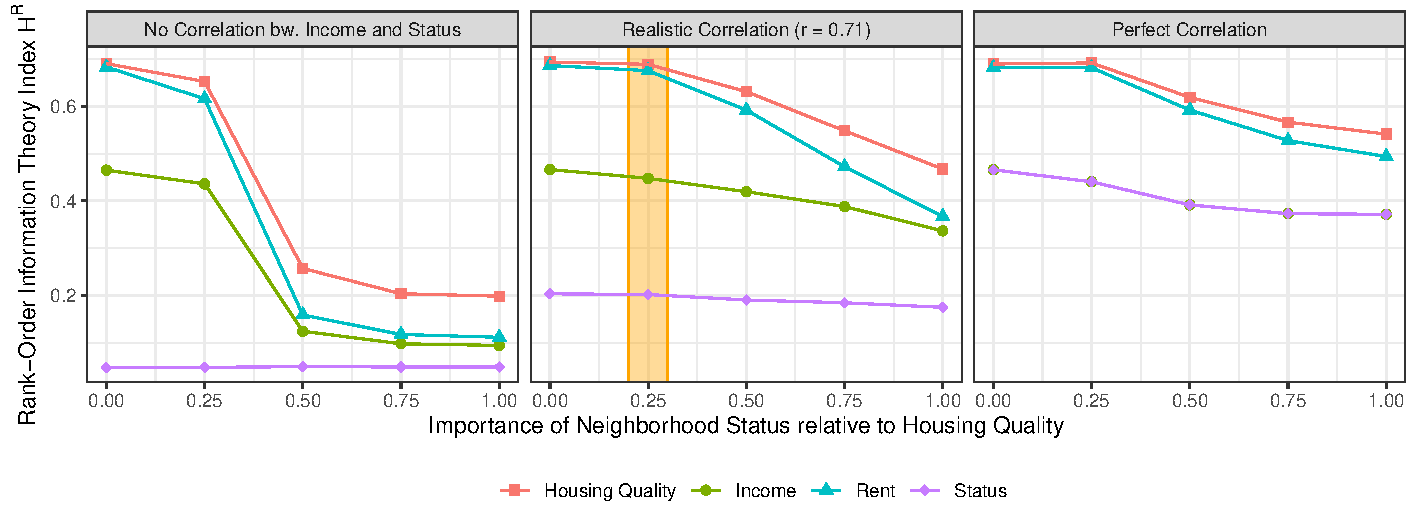
\includegraphics[width=\textwidth]{./images/abm_01_segregation}

\tiny{Segregation indices calculated for 5x5 neighborhoods and selected model parameters. The figure is based on simulated data from the main computational experiment (see Appendix A) with the following selection: $d = 0.95 \land r \in \{0, 0.5, 1\}$.} 
\label{fig:seg}
\end{figure}


Crucially, the model predicts a sizable amount of residential segregation and spatial inequality in the empirically most likely case, as shown in the highlighted area of Figure \ref{fig:seg}. Rents and housing quality are unevenly distributed across neighbourhoods in this case, while income segregation is less pronounced. Residential segregation by status is much lower but still significantly more uneven than expected by random chance. Cities self-organize into distinct and stable neighborhoods via the following mechanism: When a neighborhood increases in status, it also becomes more desirable. As desirability increases, rents increase, which triggers landlords to invest. Because the attractiveness of the neighbourhood rises with both status and housing quality, rents increase further, and the poorest residents of the neighbourhood are displaced (or poor residents can no longer afford to move to the neighbourhood). Because low incomes correlate with low status, the residents with the lowest status are likely to move out, which increases the average status of the neighbourhood. This self-reinforcing dynamic continues until the model reaches an equilibrium, where a marginal increase in neighborhood status and/or housing quality is unable to attract wealthier residents from other neighborhoods. This dynamic aligns well with the reviewed descriptions of gentrification. Conversely, if a neighbourhood decreases in status, rents tend to decrease, and landlords are less likely to invest in it. As neighborhood status and housing quality decrease, affluent households move to different neighborhoods where they can afford a higher residential satisfaction. The decreasing rent attracts less wealthy residents, for whom it is still a relatively good neighborhood. 

\begin{figure}
\caption{Residential Mobility by Income Deciles}
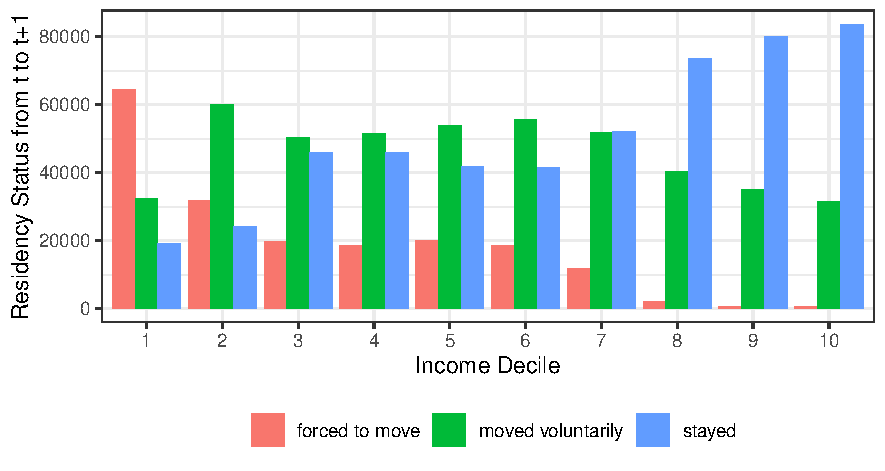
\includegraphics[width=\textwidth]{./images/abm_05_mobility}

\tiny{Frequencies of the residential status from t to t+1. If a household occupies the same housing unit in t+1 as in t, the household stayed. If the household changed the housing unit, they moved. If at t, the rent of the unit was greater than the household's disposable income, they are required to move (except if they already live in the cheapest available housing unit). If the household moved and the rent was unaffordable at t, the move is considered a forced move. The first decile has the lowest incomes, the tenth decile the highest. The figure is based on simulated data from the main computational experiment (see Appendix A) with the following selection: $a = 0.25 \land r = 0.5 \land d = 0.95$.}
\label{fig:mobility}
\end{figure}

These up- and downward spirals of neighborhoods continue until the overall city reaches an equilibrium. Once the city reaches such a stratification, where the rich reside in the best housing units in high-status neighborhoods, the richest have no incentive to move to different neighborhoods and housing units, as they cannot improve their residential satisfaction. In turn, as the most desirable places are occupied by the richest and have very high rents, the slightly less affluent households cannot improve their housing situation either and stay in the second-best houses and neighborhoods, etc. Figure \ref{fig:mobility} shows that, in equilibrium, households with high incomes are very likely to stay in the same housing unit from one point in time to the next. Households with low incomes, on the other hand, tend to move frequently. They often face unaffordable rents, even though they already live in low-quality housing units and neighborhoods (see also figure \ref{fig:quality}). When they cannot afford the rent, due to the model's design, they need to move unless they are already at the cheapest location currently available. Therefore, they move often even though their housing situation is unlikely to improve after the move. Middle-income households also exhibit lower but still considerable levels of residential mobility. However, more often than not, this move is voluntary because an affordable vacancy became available, providing them with greater residential satisfaction. Because my model incorporates population dynamics, households are randomly removed and added to the simulation, allowing vacancies to open up randomly. Because most households have a middle income, and therefore most neighborhoods are in the middle of their respective distributions, most vacancies are both available and attractive to middle-income households. Without population turnover, middle-income households would also move rarely (see robustness check B in the supplement). Although households typically do not move to improve their residential satisfaction marginally, due to life-course events, the model can reproduce the stylized fact that poor households have higher residential mobility due to affordability constraints, while middle- and high-income households move less often. If they do, they typically are not forced to do so and can improve their residential outcomes. Furthermore, the high residential mobility of low-income households, even in equilibrium, fits well with the studies that find little increased mobility of low-income households in gentrifying neighborhoods \citep{freemanDisplacementSuccessionResidential2005, dingGentrificationResidentialMobility2016, leeGeographyGentrificationResidential2023}.

\begin{figure}
\caption{Stability of the Neighborhood Hierarchy over Time}
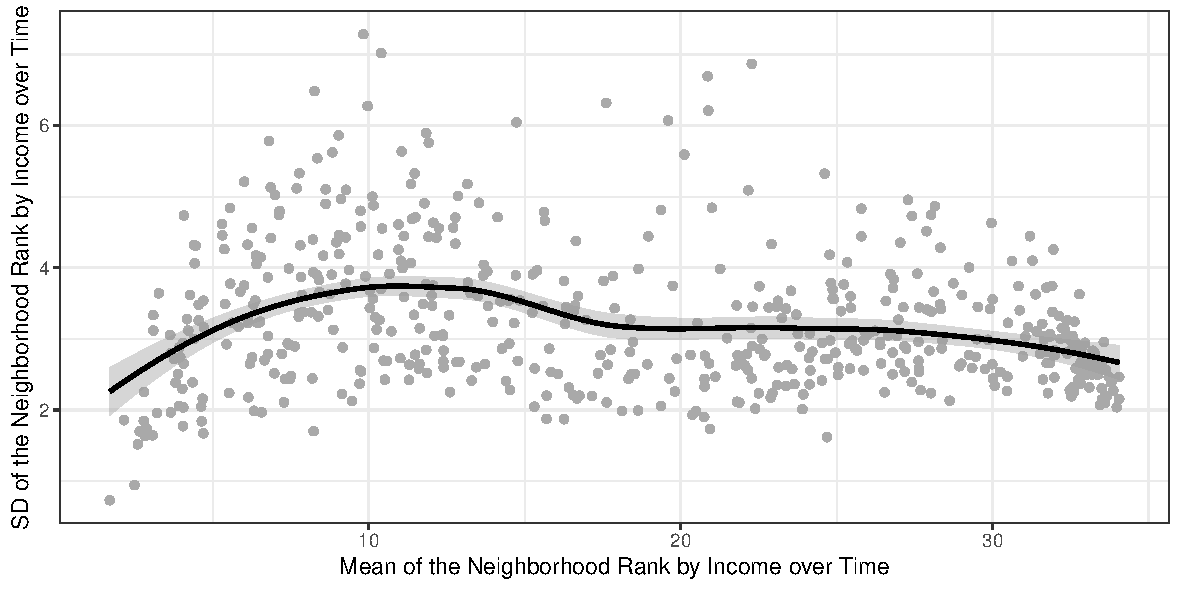
\includegraphics[width=\textwidth]{./images/abm_02b_nbstability}

\tiny{Means and standard deviations of the rank of 5x5 neighborhoods by income over time. A rank of 1 is given to the neighborhood with the highest average income at a given point in time. The figure depicts selected parameter combinations from the main computational experiment (see Appendix A) with the following selection: $d = 0.95 \land r \in \{0, 0.5, 1\}$.} 
\label{fig:stab}
\end{figure}

Despite individual residential mobility, neighborhoods are relatively stable in the empirically most plausible condition, as shown in Figure \ref{fig:stab}. It shows the standard deviation of the rank by income that a neighborhood has occupied within the city over time. Overall values are small, particularly compared to some parameter combinations where no segregation emerges and no stable neighborhoods form. Nevertheless, there is some variation in neighborhood ranks, primarily triggered by population turnover again (see supplement: robustness check B). However, in line with the stylized facts again, there is an inverse-U-shaped relationship between the variation in income ranks and the average income rank: neighborhoods at the top and bottom of the income distribution tend to be more stable than those in the middle. The curvature is less visible in conditions with overall high stability. However, in conditions with slightly lower overall stability, this relationship becomes very apparent (see supplement).

\begin{figure}
\caption{Household Income, Rent, and Housing Quality}
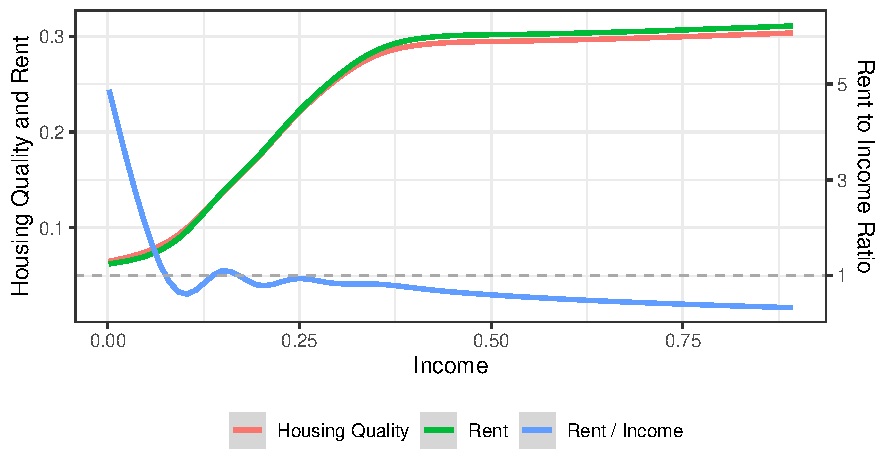
\includegraphics[width=\textwidth]{./images/abm_03_inequality}

\tiny{LOESS smoothers for the relationship between housing quality, rent, and the rent-to-income ratio with household income in the empirically most plausible parameter combination. The figure is based on simulated data from the main computational experiment (see Appendix A) with the following selection: $a = 0.25 \land r = 0.5 \land d = 0.95$.} 
\label{fig:quality}
\end{figure}

As discussed in the mechanism leading to segregation, high-income households can outcompete other households for the most desirable housing units. Figure \ref{fig:quality} confirms this relationship on the individual level: there is a positive relationship between household income and both the rent they pay for the housing unit and the quality of the housing unit. However, the slope of this relationship decreases as income increases. While the absolute rent and housing quality (and neighborhood status, see robustness check C) increase with income, the relative increase slows down. The result is the observation that wealthier households pay more in absolute terms but a lower proportion of their income for housing. In contrast, it is common for low- to middle-income households to live in housing units where rent exceeds their (disposable) income, even though they live in cheap, low-quality neighborhoods and housing units. But why are the rents of the worst housing units still higher than the disposable incomes of the poorest? As rent is set globally based on utility, there is no exploitation on behalf of landlords in this model. They do not set prices. The reason is easiest to understand when considering neighborhood status: because neighborhood status is, by definition, an average of the individual status of residents in a neighborhood, the distribution of neighborhood status has lower variance than the individual status distribution. Because landlords invest in housing quality based on the average rent in the neighborhood, there is a reduction in variance in housing quality compared to rents as well. So, for both components of the utility function, there is a reduction in variance because they depend on averages. The distribution of housing units by utility is less unequal than the income distribution of households. For wealthy households, this limits the supply of desirable units, which is a reason why the rich pay a lower share of their income for housing\footnote{This result could also be due to the specification of the utility provided by a unit (Appendix A, equation \ref{eq:util}). It is a common assumption in economics that marginal utility is decreasing. When a household already resides in a high-quality housing unit, the added utility provided by a specific increase in housing quality is lower than the added utility of the same change in housing quality when the household lives in a housing unit of lower quality (and the same holds for neighborhood status). As a consequence, households are less willing to pay more rent for improved housing quality and a better neighborhood status. Moreover, the choice of using the 75th percentile in the rent formula could contribute to the slowing down of the relationship between household income and utility.}. However, for the poorest, this means that no housing units are supplied that are of such low quality that they could afford them. 

\begin{figure}
\caption{Regression of Housing Quality on Status and Income}
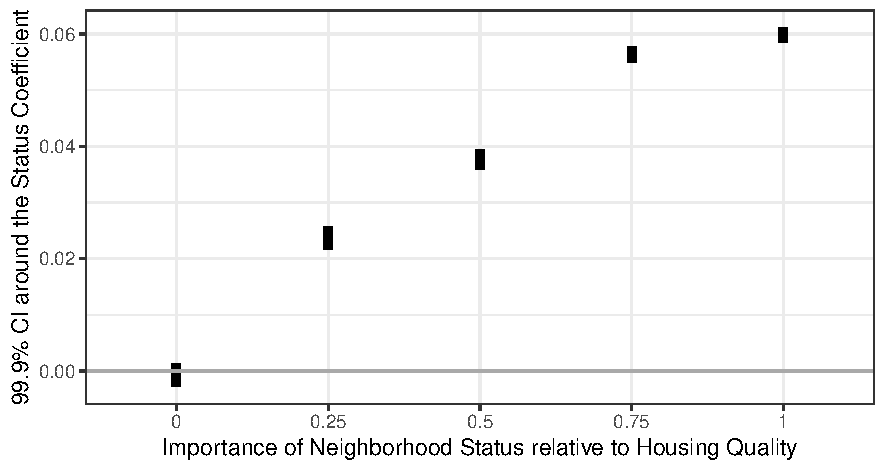
\includegraphics[width=\textwidth]{./images/abm_04_statusreg}

\tiny{Confidence intervals for the coefficient of status in separate OLS regressions of housing quality on household income and status. Each regression is calculated using one set of parameters, where only the importance of neighborhood status is varied, and the other parameters are held constant at their most plausible values. Because the agents in the model are interdependent, the IID assumption of the OLS regression is violated, resulting in downward-biased standard errors. The figure is based on simulated data from the main computational experiment (see Appendix A) with the following selection: $r = 0.5 \land d = 0.95$.}
\label{fig:reg}
\end{figure}

Because status and income are correlated, it is no surprise that low-status households tend to reside in poorer neighborhoods and substandard housing units. However, existing empirical research has shown that minorities often have worse residential outcomes even after controlling for their income. As discussed above, landlords cannot set prices in this model and, therefore, this model cannot reproduce price discrimination. Nevertheless, it can (partially) explain inequality in housing quality by status after controlling for income. Figure \ref{fig:reg} shows the OLS confidence intervals for status from multiple regressions of housing quality on household status and income. We observe a significantly positive relationship between status and housing quality after controlling for income, which increases as households value neighborhood status more in their location choice. High-status households tend to live in higher-quality housing units, and low-status households live in lower-quality housing units, independent of income. The reason for this observation within this model is that when a low-status household moves to a neighborhood, the attractiveness of that neighborhood and, consequently, its rents decrease. When rents decrease, landlords tend to refrain from investing, resulting in a deterioration of housing quality. The same mechanism holds in reverse: a high-status household increases neighborhood attractiveness and rents, which leads landlords to invest in a higher housing quality. This result aligns well with empirical studies on racial discrimination in the US, where a frequent concern among existing residents is that housing values will decrease when minority members move to the neighborhood \citep{harrisPropertyValuesDrop1999, krysanDoesRaceMatter2009}.


\section{Limitations}

This model, like any theoretical model, has omissions and limitations that must be acknowledged. This model's most important scope condition is that housing needs to be allocated via markets. The reviewed literature primarily focuses on North America and Western Europe, so the stylized facts explained by this model may be geographically limited. Even within these contexts, this model makes noteworthy assumptions. First, this model does not consider strategic action and exploitation \citep{desmondPoorPayMore2019}. It is noteworthy, however, that this model is nonetheless able to explain patterns of housing inequality and unaffordability. I am not suggesting that there is no exploitation in housing markets, but inequalities might persist without exploitative practices. Second, we know that land and housing are often used as assets and investment properties; therefore, housing supply depends on macroeconomic conditions \citep{bayerSpeculativeFeverInvestor2021}, which I have omitted from this model for simplicity. Macro-economic conditions could make it more or less profitable to invest in housing stock and, therefore, be a trigger for neighborhood change. Third, I also omitted geographical features and distance to amenities. I abstracted from exogenous amenities in my model to highlight the endogenous processes at work that sustain segregation and lead to changes in neighborhoods due to shocks. Although this provides many insights into these processes and can explain multiple stylized facts, it is fundamentally aspatial. It overlooks a substantial body of literature that documents the importance of amenities. These could further explain where groups segregate to \citep{gaigneWhoLivesWhere2022} and which neighborhoods change \citep{leeNaturalAmenitiesNeighbourhood2018}. Zoning has also been omitted, not just for simplicity but also due to endogeneity. Particularly, density zoning is a way to institutionalize areas where poor households cannot afford to move to; such laws likely stem from affluent households' preferences to keep the poor out of their areas \citep{rothwellDensityZoningClass2010}.

The process of moving is also highly stylized. In reality, searching for housing or new occupants takes time, is connected to transaction costs, depends on the availability of information, often involves intermediaries like real estate agents, and households might be discriminated against \citep{hanMicrostructureHousingMarkets2015}. Households typically move around life-course events, rather than marginally increasing their utility. Some sociologists have recently called for more realistic micro-foundations of theoretical models of residential stratification. Particularly, they review and present evidence that households first heuristically narrow down the neighborhood in which they search for a housing unit before assessing the qualities of available units more rationally \citep{krysanCycleSegregationSocial2017, bruchChoiceSetFormation2019}. However, the general assumption that households want to find a high-quality unit in a high-quality neighborhood but are constrained by their budget remains plausible (although there is some heterogeneity in preferences and decision-making), and the less realistic depiction of the housing search process simplifies the model and keeps it in line with economic theory. There are two ways, however, in which the utility maximization assumption may contribute to substantial shortcomings of the model. First, when households consider neighborhood and housing quality at different stages of the search process, these goods are not substitutes. It is, however, hard to say if this leads to over- or underestimation of segregation. Second, utility maximization models cannot explain the established causal link between increasing income inequality and increasing income segregation (see robustness check C). \citet{yavasDissectingIncomeSegregation2019} has suggested a formal model that can explain this link with a bounded rationality approach. Increased inequality leads to larger absolute differences between neighborhoods, which increases the probability that households make a segregating move.

%This model deliberately concentrated on socio-economic segregation with little reference to racial/ethnic segregation. But it could be extended similarly to the models by \citet{masseyAmericanApartheidSegregation1993, bruchHowPopulationStructure2014}, where ethnic inequality and economic segregation interact, explaining patterns in ethnic segregation. Although there is a large body of work that documents how race and ethnicity shape residential segregation and neighborhood change in the US (e.g., \cite{hwangUnequalDisplacementGentrification2020}), these results are likely not generalizable as the history of racial relations and institutionalization of racial boundaries in the US is very specific. The extent to which racial and ethnic composition plays a role in residential segregation in other contexts beyond economic disadvantage is underresearched.

\section{Conclusion}

%Existing scholarship on the role of landlords in housing inequality and segregation has been concerned with discrimination as a reason for segregation and inequality \citep{charlesDynamicsRacialResidential2003}. In particular, there have been two theories of discrimination that have been applied to housing as well \citep{auspurgClosedDoorsEverywhere2019}: taste-based and statistical discrimination. Taste-based discrimination refers to to a landlord/realtor that dismisses applications from households with sufficient funds based on their group membership and is willing to accept costs from dismissing potential customers. Economists have often seen this type of discrimination as inefficient and that market competition should make this type of discrimination less prevalent \citep{arrowWhatHasEconomics1998}. Another strand of theory, and a partial response to this observation, has been statistical discrimination where the landlords uses group membership as proxy. This theory has proven the possibility a third reason of apparent discrimination in housing which in existing tests cannot be distinguished from taste-based discrimination on behalf of landlords. But when households value their neighborhood, renting to minority households decreases local rents and makes investments less attractive. With lower investments into housing quality, minority neighborhoods will be of lower quality even if there is sufficient income. And the other way around, minority households need to pay a premium to achieve a similar residential outcomes to offset their effect on the neighborhood. Similar arguments have been made in labor markets where employers might fear that their existing workforce opposes hiring minority members \citep[95]{arrowWhatHasEconomics1998} and aligns with the observed concern among existing residents that housing values will decrease when minority members move to the neighborhood \citep{harrisPropertyValuesDrop1999, krysanDoesRaceMatter2009}. 

The proposed theoretical model extends existing models of residential segregation and housing inequalities. By incorporating the characteristics of housing units and the agency of landlords into neighborhood composition, the model extends beyond existing explanations that primarily emphasize demand-side factors \citep{desmondPoorPayMore2019, rosenthalChangePersistenceEconomic2015}. This addition is crucial, as empirical research suggests that households often prioritize features of their homes—such as quality and affordability—over the surrounding neighborhood's amenities or demographics. Ignoring the built environment's role in explaining residential segregation and neighborhood change misrepresents the motives and behaviors of households. The model shows that both households' neighborhood preferences and spatially contingent investments can create sizable levels of segregation (even without the presence of the other). When both mechanisms are at work, they can reinforce each other and create stable segregated neighborhoods by income, social status, as well as rent and housing quality. Moreover, the insights gained from this model reveal that the mechanisms underlying residential segregation and neighborhood change are intrinsically linked to patterns of residential mobility and housing inequality. By considering housing quality in segregation models, these models become more realistic (they better reflect household preferences) and more general (they explain a wider range of phenomena). This model, therefore, represents a crucial step toward a more comprehensive synthesis of urban theory.

%\section{Implications for Policy}

%Ghettos and very disadvantaged nbs are a result of the general workings of thehousing market, therefore place-based policies will not work. to prevent extremes, one needs to combat segregation as a whole. but how? if characteristics of the dwelling are most important, one could try to foster mixed housing: mandate investors to build different sized and priced housing units in the same building in rich areas, programs to reduce investment uncertainty in poor areas, mixed zoning etc.

%In this theory, I take the position that neighborhood change is not a phenomenon on the neighborhood level but a manifestation of a shift in spatial equilibrium caused by external shocks like income or population increases (like e.g. \cite{galsterNatureNeighbourhood2001, leeNaturalAmenitiesNeighbourhood2018}). Neighborhood change is therefore caused by changes to the city as a whole but the workings of the housing market concentrate the resulting changes in space. I therefore disagree with \citet[358]{hwangUnequalDisplacementGentrification2020} who observe that "gentrification reduces the overall pool of neighborhoods accessible to financially disadvantaged residents within the city". Not gentrification "causes" less affordable housing, shocks in population and income cause it. Gentrification is the process by which it does. If we would try to protect individual neighborhoods, the increase in demand would simply create displacement elsewhere. Nonetheless, as moving includes transaction costs and displacement primarily affects the poor, there is indeed a social injustice connected to gentrification. But place-based policies will not work as demand will seek its supply somewhere else (\textit{substitution effect}). Gentrification should less be a concern in its own right but city-wide housing supply should, and particularly housing elasticity. 



\section*{Appendix A: The Agent-based Model}

I formalize the theoretical argument using an agent-based model, where agents interact on a regular spatial grid, as popularized by \citet{schellingDynamicModelsSegregation1971}. There are two classes of agents that interact with each other and themselves. Households occupy housing units and want to live in those housing units that maximize their residential satisfaction, i.e. utility, which is a function of housing quality and neighborhood status, given their budget. They are mobile, so they can move in and out of housing units and neighborhoods if there are vacant units. Landlords own the housing units, which are represented by the cells on the city grid. They need to decide whether it is profitable to invest in their housing units, which they do heuristically based on changes in rents in the neighborhood.

\subsection*{Modeling Demand}

Households are the demanders of housing. Each household $i$ is characterised by their income disposable on housing $w_i \in [0, 1]$ and their social status $s_i \in [0, 1]$. Both household attributes are fixed over time. Income distributions are almost always positively skewed and long-tailed. I sample the household's income from a $Beta(2, \ 5)$ distribution in the main experiment to capture this typical feature. Income inequality in samples from this distribution, as measured by the Gini index, averages about 31.5, which is comparable to the level of income inequality in Germany, France, and Canada in recent years\footnote{World Bank Poverty and Inequality Platform: \url{https://data.worldbank.org/indicator/SI.POV.GINI/}}. I use different Beta distributions in robustness check C. I assume a similar distributional form for social status $s_i$, which is typically correlated with income. The social status is therefore sampled dependent on income and a correlation parameter $r \in [0, 1]$: 

\begin{equation}
 s_i \sim r \ w_i \\ + \\ (1 - r) \ Beta(2, \ 5)
\end{equation}
\label{eq:soc}

Housing in this model represents a consumption bundle $x$ of two commodities, housing quality $q(x, t)$ and neighborhood status $\bar{s}(x, t)$, which are variable over time $t$. Housing quality is variable because landlords can invest (see section on supply), and neighborhood status is variable over time as households can move into and out of units and neighborhoods. Housing quality represents the desirability of the unit, while neighborhood status represents the desirability of the neighborhood. I operationalize neighborhood status as the average social status of the inhabitants $j$ of the housing units in the Moore neighborhood of the housing unit $x$ that household $i$ considers moving to at time $t$. $n_{x, t}$ is the number of neighbors the household would have at that location, i.e., the number of occupied housing units neighboring $x$ at time $t$. Robustness check D varies the size of these Moore neighborhoods. The social position of a neighbor $j$ at location $x$ at time $t$ is referred to by $s_{j}(x, t)$. 

\begin{equation}
 \bar{s}(x, t) = \frac{1}{n_{j}(x, t)} \sum_{j = 1}^{n_{j}(x, t)} s_{j}
\end{equation}
\label{eq:status}

I propose the following Cobb-Douglas utility function to model the household's housing preferences. The parameter $a \in [0, 1]$ weighs the two commodities and expresses how important social preferences are relative to housing quality. If $a = 0$, only housing quality matters in the utility calculation of the household; at $a = 1$, only average social status matters. $a$ is identical for all households in a given simulation run, therefore, all housing units are equally desirable to all households.

\begin{equation}
 U(x, t) = \\ \bar{s}(x, t)^a \\ q(x, t)^{1-a}
\end{equation}
\label{eq:util}

The set of all housing units $x$ at time $t$ is denoted by $X(t)$, and the set of renters inhabiting housing unit $x$ at time $t$ is denoted $L(x, t)$, which can contain at most one renter: $|L(x, t)| \leq 1 \ \forall \ x, t$. For each household $i$, there is a set of available options, the \textit{budget set} $B_i(t) \subseteq X(t)$. The housing units in this set are the household's current and unoccupied locations if the rent $p(x, t)$ of these locations is less or equal the household's disposable income. If the current location becomes too expensive for the household, it is no longer within the budget set, and the household is forced to move, i.e. the household is displaced. 

\begin{equation}
B_i(t) = \{x \in X(t): (\ L(x, t) = \{\emptyset\} \ \lor \ L(x, t) = \{i\}) \ \land \ p(x, t) \leq w_i \}
\end{equation}

Suppose households choose their housing unit according to the discussed preferences. In that case, their choice of housing unit $x$ can be treated \textit{as if} they maximize their utility under the constraint that they need to be able to afford this location:

\begin{equation}
\operatorname*{arg\,max}_{x \in B_i(t)} U(x, t) \\*
\end{equation}

If no housing units are available with rent below or equal to the household's disposable income, the household moves to the empty location with the lowest rent. 


\subsection*{Modeling Supply}

Landlords supply housing quality $q(x, t)$ of housing unit $x$. $q(x, t)$ represents the monetary value of housing quality independent of the neighborhood. Quality is path-dependent; it is dependent on past investments. Landlords invest in their housing quality if the average rent in the Moore neighborhood increases. As landlords would like to know whether investing will be profitable, an increase in average neighborhood rent indicates that their neighborhood attracts wealthy residents who are able to provide a return on investment. However, if the rents in the neighborhood decrease, returns in this neighborhood are too low to justify investments.

As $q(x, t)$ represents the monetary value of housing quality, landlords set housing quality equal to the average neighborhood rent if they invest. This also reflects that landlords are responsive to the size of the change in neighborhood incomes. If neighborhood incomes only rise slightly, they will not invest large sums of money. If they do not invest, housing quality decays exponentially. The decay parameter $d \in [0, 1[$ gives the proportion of housing quality a unit retains after one time step without investment. 

If $x_j$ is one of the $n_v$ housing units in the Moore neighborhood (the size of the Moore neighborhoods are varied in robustness check D) of housing unit $x_i$ at time $t$, the average rent $\bar{p}(x_i, t)$ in the neighborhood of $x_i$ at time $t$ is given by:

\begin{equation}
\bar{p}(x_i, t) = \frac{1}{n_v} \sum_{k = 1}^{n_v} p(x_j, t)
\end{equation}

\begin{equation}
q(x_i, t) = 	\begin{cases}
			\bar{p}(x_i, t) & \bar{p}(x_i, t) \geq \bar{p}(x_i, t-1) \\
			d * q(x_i, t-1) & \bar{p}(x_i, t) < \bar{p}(x_i, t-1)
			\end{cases}
\end{equation}
\label{eq:quality}

\subsection*{Rent}

$C(x_i, t)$ denotes all housing units $x_j$ that have a lower utility than $x_i$, which are the competition of $x_i$. Rent is then the 75th percentile of incomes of the households $L(C_i)$ living in the housing units in the competition set.

\begin{equation}
C(x_i, t) = \{ x \in X: U(x_j, t) \leq U(x_i, t)  \}
\end{equation}

\begin{equation}
p(x, t) = P_{75}[\{ L(C_i): w_i  \}]
\end{equation}


\subsection*{Simulation Experiments}


\begin{table}[h!]
  \centering
  \caption{Parameters of the Main Computational Experiment}
  \begin{tabularx}{\textwidth}{l l X}
    \hline
    \textbf{Parameter} & \textbf{Values} & \textbf{Description} \\
    \hline
    $a$ & 0, 0.25, 0.5, 0.75, 1 & The importance of neighborhood social status relative 						to the importance of housing quality in households' 							utility function. 0 means only housing quality 									matters, 1 implies that only neighborhood status 								matters. See equation \ref{eq:util}. \\
    $r$ &  0, 0.25, 0.5, 0.75, 1 & Correlation of households' income and social status. 						When $r$ is 1 , status and income are identical. See 							equation \ref{eq:soc}. \\
    $d$ & 0.95, 0.9, 0.85, 0.8 & Rate of decay of housing quality when landlords do not invest. 				$d$ gives the proportion of housing quality that is retained 				from one time step to the next without investments. See 						equation \ref{eq:quality}. \\
    size & 30 & Edge length of the grid. \\
    density & 0.85 & Population density: which proportion of the housing units are occupied by households. \\
    distribution & 2 & This value determines the shape of the Beta distribution used to sample household income and status. These variables are sampled from a 	Beta(distribution, 2.5 x distribution) probability density function to model different levels of inequality in income and status. This parameter is varied in robustness check C.\\
    turnover & 0.02 & This parameter introduces noise to the model via 							population dynamics. It is the percentage of households that move out of the city. A corresponding number of households move into the city to keep the population constant. This parameter is varied in robustness check B.\\
    vision & 1 & Size of the Moore neighborhoods agents consider when calculating average status and rent during the simulation. This parameter is varied in robustness check D. \\
    steps & 400 & The number of time steps the simulations run. \\
    iterations & 15 & Number of times each combination of parameters is run.\\
    (size nb) & 5 & Edge length of the neighborhoods which are used to calculate segregation indices and neighborhood averages in the analysis. \\
    \hline
    \end{tabularx}%    
  \label{tab:parameters}%
\end{table}%

Housing units and their landlords are immobile, represented by 900 squares representing a city on a 30x30 toroidal lattice. Households can move between these housing units if another household does not occupy them. About 85\% of the housing units are occupied by households. 

Because randomness affects the results of computational models \citep{macySignalImportanceNoise2015} and stochastic models are empirically more accurate \citep{masRandomDeviationsImprove2020}, I add random moves. Each household has a two percent chance of moving out of the city. A corresponding number of newly created households move into the city, so vacancy rates remain identical over time.

I ran 15 simulations with the same parameter combinations for the main results. I use five levels in the parameters $a$ and $r$: 0, 0.25, 0.5, 0.75, and 1. $d$ is varied in four levels: 0.95, 0.9, 0.85, 0.8. Each combination of parameters is repeated 15 times. This results in 1500 simulation runs of 400 time steps each. Each simulation outputs a time series of every housing unit and household, resulting in 1500 runs x 400 time points x 900 housing units = 540 million observations of housing units in the raw data set.

For more details on the models parameters and which other parameters I have varied in robustness checks, see table \ref{tab:parameters} and the supplementary material.

% TODO add pseudo code

\subsection*{Measurement and Analysis}

In the presented analyses, I only analyse data after the burn-in period, when the model already converged to a steady equilibrium. In the main experiment, I analyse the last 100 time steps out of the simulated 400. The analysis sample therefore consists of 135 million observations of housing units and their occupying households.

In data preparation, I generate two additional data sets from the observations of housing units. I cut the grid into 5x5 neighborhoods for analysis before calculating segregation indices for every time point and every simulation run based on these neighborhoods. As most of my variables are continuous, I categorize them using deciles and calculate the rank-order information theory index $H^R$ \citep{reardonNewApproachMeasuring2006} for income, status, rents and housing quality. These aggregate indices and Gini indices for the overall levels of inequality in the endogenous variables rent and housing quality are saved in a data set representing the city level. I also export a neighborhood level data set with averages in all relevant variables and their rank order to assess stability and changes of neighborhoods. I merge the neighborhood averages to the individual level data to analyse who is living in which neighborhoods and calculate some individual level indicators such as the ratio between rent and income.

For more details on the performed analyses and their interpretations, see the supplementary materials and the respective Python and R code.

%\section*{Appendix B: Observable Implications \textcolor{red}{(tbc)}}

%\begin{enumerate}
%	\item Neighborhoods are more homogenous in housing quality (and rent?) than in income and status.
%	\item Cities are more segregated, the more income and status are correlated.
%	\item Cities are more segregated, the more housing quality matters to households.
%	\item Correlation and preferences interact in their relation to segregation.
%	\item Neighborhoods are more stable over time in more segregated cities.
%	\item More segregated cities have higher inequalities in housing quality and rent.
%	\item There is a decrease in marginal return of housing quality by income.
%	\item The very poor are less residentially mobile than the poor but more than the rich.
%	\item The more segregated the city, the less residentially mobile are the middle and high income households.
%	\item Ratio between rent and income between different levels of segregation?
%	\item The more important neighbors status is to households, the lower the housing quality of low status residents even when controlling for income.
%	\item The more segregated a city by income, the more concentrated are vacancies in the poorest and most rundown neighborhoods.
%	\item the more segregated a city, the stronger is the correlation between income and housing quality.
%\end{enumerate}



\singlespacing
\printbibliography

\end{document}
